% ID: SEL-D0016-BA-E01
% ESTADO: validada. S017. Revisión matemática, didáctica y visual.
\textbf{Variables, restricciones y beneficio.}\par\nopagebreak[4]
Sean $x$ e $y$ los kilogramos de Delicia Roja y Delicia Negra. Las cantidades son reales y deben satisfacer
\[
3x+y\leq15,\qquad x+2y\leq10,\qquad y\geq\frac32,\qquad y\leq2x,\qquad x\geq0.
\]
Las primeras desigualdades corresponden a fresas y chocolate. Se maximiza $F(x,y)=3x+5y$, en euros.

\textbf{Recinto y solución.}\par\nopagebreak[4]
El recinto resulta de intersectar los semiplanos. En orden, sus vértices son
\[
(3/4,3/2),\quad(9/2,3/2),\quad(4,3),\quad(2,4).
\]
Se cortan sucesivamente las fronteras $y=2x$ y $y=3/2$, la horizontal con $3x+y=15$, las dos de recursos y, por último, $x+2y=10$ con $y=2x$. En esos puntos, $F$ vale $39/4$, $21$, $27$ y $26$.
\begin{center}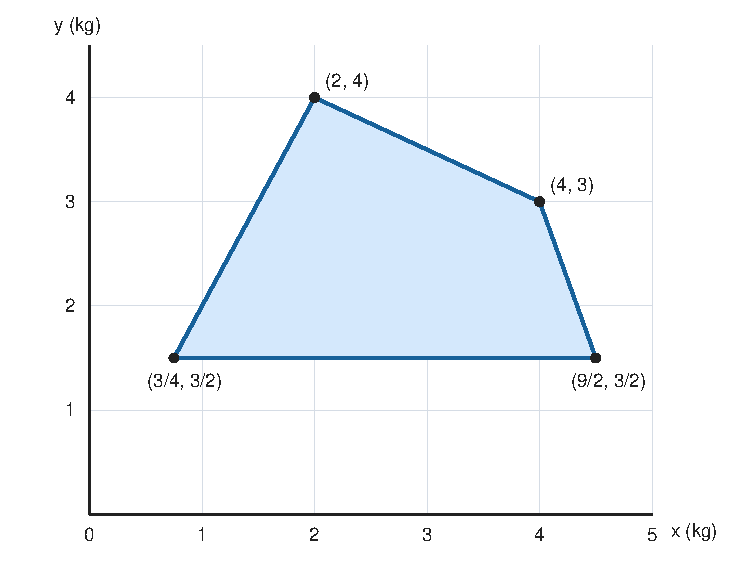
\includegraphics[width=0.53\linewidth]{recursos/figuras/s017-region.pdf}\end{center}
La cota global
\[
3x+5y=\frac15(3x+y)+\frac{12}{5}(x+2y)\leq27
\]
se alcanza al agotar ambos recursos. El punto $(4,3)$ cumple las demás restricciones, por lo que el máximo es único.
\[
\boxed{4\text{ kg de Delicia Roja},\qquad3\text{ kg de Delicia Negra},\qquad27\text{ euros}.}
\]
